% SPDX-License-Identifier: AGPL-3.0-or-later
% Commercial license available
% © Concepts 1996-2026 Miroslav Sotek. All rights reserved.
% © Code 2020-2026 Miroslav Sotek. All rights reserved.
% ORCID: 0009-0009-3560-0851
% Contact: www.anulum.li | protoscience@anulum.li
% scpn-quantum-control --- Phase 3 entanglement/tomography short paper

\documentclass[preprint,aps,physrev,superscriptaddress,floatfix,longbibliography]{revtex4-2}

\usepackage{amsmath,amssymb}
\usepackage{booktabs}
\usepackage{graphicx}
\usepackage{hyperref}
\usepackage{xcolor}
\usepackage{xurl}
\usepackage{siunitx}

\hypersetup{
    colorlinks=true,
    linkcolor=blue!60!black,
    citecolor=blue!60!black,
    urlcolor=blue!60!black,
}

\begin{document}
\emergencystretch=3em

\title{Reduced-Pauli entanglement checks for DLA-sector leakage mechanisms on IBM Heron hardware}

\author{Miroslav \v{S}otek}
\email{protoscience@anulum.li}
\affiliation{ANULUM, Marbach SG, Switzerland}
\affiliation{ORCID: 0009-0009-3560-0851}

\date{\today}

\begin{abstract}
Parity-sector leakage asymmetry in small Kuramoto--XY circuits is a useful
hardware observable only if the mechanism can be separated from layout,
prepared-state, and readout artefacts. We report a cost-bounded reduced-Pauli
entanglement/tomography check for promoted Phase~3 DLA-parity and
Fisher-information-modified Kuramoto--XY circuit families. The approved
\texttt{ibm\_marrakesh} execution used physical qubits $[1,2,3,4]$, 162 main
circuits, four readout calibration circuits, 2048 shots per main circuit, and
8192 shots per readout circuit. The submitted IBM jobs were
\texttt{d86g7h1789is738vkreg} and \texttt{d86ggpis46sc73f6v170}. A
preregistered reducer produced 54 observable rows. The mean absolute
measured-minus-exact deviation is 0.1299 and the maximum absolute deviation is
0.5561. The largest deviations are concentrated in transverse two-qubit
correlators, especially DLA odd-sector \texttt{XX}/\texttt{YY} edge channels,
while the FIM $\lambda_{\mathrm{fim}}=4$ circuit deviates more strongly than
the $\lambda_{\mathrm{fim}}=0$ reference. The result is a mechanism-boundary
measurement: it shows structured reduced-Pauli distortions accompanying the
small-system DLA/FIM hardware programme, but does not claim scalable
tomography, quantum advantage, full-state reconstruction, or backend-general
entanglement dynamics.
\end{abstract}

\maketitle

\section{Introduction}

Kuramoto synchronisation and XY spin Hamiltonians provide a compact route from
phase-oscillator structure to gate-model quantum dynamics~\cite{Kuramoto1975,Acebron2005}.
In the present programme, the relevant small-system hardware question is not
whether a broad advantage has been demonstrated. It is narrower: when
sector-resolved leakage and retention observables deviate from exact
Kuramoto--XY references on IBM hardware, do reduced-Pauli correlators show an
accompanying structure that can constrain the mechanism?

Previous DLA-parity and FIM runs established bounded hardware observations,
including backend, layout, state-preparation, and readout sensitivity. A scalar
leakage metric alone cannot distinguish coherent correlator deformation from
population readout effects or generic depth-dependent decoherence. This paper
therefore measures a small set of preregistered reduced-Pauli observables for
the same class of promoted circuits. Full tomography is unnecessary for this
question: the aim is to compare selected two-qubit correlators against exact
classical references under one backend, layout, shot budget, and calibration
window.

\section{Protocol}

The source circuits are listed in Table~\ref{tab:sources}. Four DLA-parity
circuits compare even and odd initial states at shallow and signal depths. Two
FIM-pair circuits compare $\lambda_{\mathrm{fim}}=0$ and
$\lambda_{\mathrm{fim}}=4$ at fixed initial state and depth.

\begin{table}[tb]
\centering
\begin{tabular}{lllc}
\toprule
Label & Family & Initial state & Depth \\
\midrule
\texttt{dla\_even\_shallow} & DLA parity & \texttt{0011} & 6 \\
\texttt{dla\_odd\_shallow} & DLA parity & \texttt{0001} & 6 \\
\texttt{dla\_even\_signal} & DLA parity & \texttt{0011} & 10 \\
\texttt{dla\_odd\_signal} & DLA parity & \texttt{0001} & 10 \\
\texttt{fim\_lambda0\_reference} & FIM pair & \texttt{0011} & 4 \\
\texttt{fim\_lambda4\_feedback} & FIM pair & \texttt{0011} & 4 \\
\bottomrule
\end{tabular}
\caption{Promoted source circuits for the reduced-Pauli check.}
\label{tab:sources}
\end{table}

For each source circuit we measure nine reduced-Pauli basis settings,
\begin{equation}
\{\texttt{IIXX},\texttt{IIYY},\texttt{IIZZ},\texttt{IXXI},\texttt{IYYI},
\texttt{IZZI},\texttt{XXII},\texttt{YYII},\texttt{ZZII}\}.
\end{equation}
Each source/basis pair is repeated three times at 2048 shots, giving 162 main
circuits. Four computational-basis readout states, \texttt{0000},
\texttt{0001}, \texttt{0011}, and \texttt{1111}, are measured at 8192 shots.
The complete hardware block therefore contains 166 circuits. The selected
physical qubits are $[1,2,3,4]$ on \texttt{ibm\_marrakesh}; the maximum
transpiled depth in the live preflight is 388, and the maximum
measurement-basis depth expansion is 1.0718.

\section{Analysis}

For each measured basis-rotated circuit, the reducer estimates the Pauli
expectation
\begin{equation}
  \langle P \rangle =
  \frac{1}{N}\sum_b n_b
  \prod_{i\in \mathrm{supp}(P)} (-1)^{b_i},
\end{equation}
where $P$ is the reduced-Pauli label, $n_b$ is the observed count for bitstring
$b$, and $N$ is the total shot count. Repetitions are grouped by source label
and basis setting, then compared with exact reference expectations from the
committed reference table
\path{data/phase3_entanglement_tomography/entanglement_observable_rows_2026-05-07.csv}.

The primary output rows are committed in
\path{data/phase3_entanglement_tomography/entanglement_tomography_rows_2026-05-20.csv}.
The rows have SHA256 digest
\path{3d18308d60fe32827bae7517f18fd71690240b105779287408c4749cb0e7dc72}.

\section{Results}

The approved IBM execution completed on \texttt{ibm\_marrakesh}. The submitted
jobs were \texttt{d86g7h1789is738vkreg} and
\texttt{d86ggpis46sc73f6v170}. The analysis produced 54 observable rows with
mean absolute deviation 0.1299 and maximum absolute deviation 0.5561 relative
to exact references.

Table~\ref{tab:label-summary} gives the label-level aggregates. DLA circuits
have larger mean absolute deviation than the FIM pair overall. Within the DLA
family, the odd shallow and odd signal circuits produce the largest aggregate
departures. Within the FIM pair, $\lambda_{\mathrm{fim}}=4$ has more than twice
the mean absolute deviation of $\lambda_{\mathrm{fim}}=0$.

\begin{table}[tb]
\centering
\small
\begin{tabular}{lrrr}
\toprule
Circuit label & Mean signed & Mean absolute & Max absolute \\
\midrule
\texttt{dla\_even\_shallow} & -0.120474 & 0.148396 & 0.314180 \\
\texttt{dla\_even\_signal} & 0.061095 & 0.063458 & 0.160443 \\
\texttt{dla\_odd\_shallow} & 0.098416 & 0.219708 & 0.515473 \\
\texttt{dla\_odd\_signal} & 0.153497 & 0.176026 & 0.556091 \\
\texttt{fim\_lambda0\_reference} & 0.030496 & 0.052205 & 0.088148 \\
\texttt{fim\_lambda4\_feedback} & 0.096107 & 0.119566 & 0.274155 \\
\bottomrule
\end{tabular}
\caption{Label-level measured-minus-exact deviation aggregates. Each row
summarises nine reduced-Pauli observables.}
\label{tab:label-summary}
\end{table}

Figure~\ref{fig:heatmap} shows the signed measured-minus-exact deviations by
source label and basis setting. The strongest pattern is not a uniform decay of
all correlators. Instead, deviations concentrate in transverse two-qubit
channels. The odd-sector DLA signal circuit has large positive shifts in
\texttt{XXII} and \texttt{YYII}; the odd shallow circuit has analogous positive
shifts in \texttt{IIXX} and \texttt{IIYY}. The even shallow circuit moves in
the opposite direction on corresponding transverse channels.

\begin{figure}[tb]
\centering
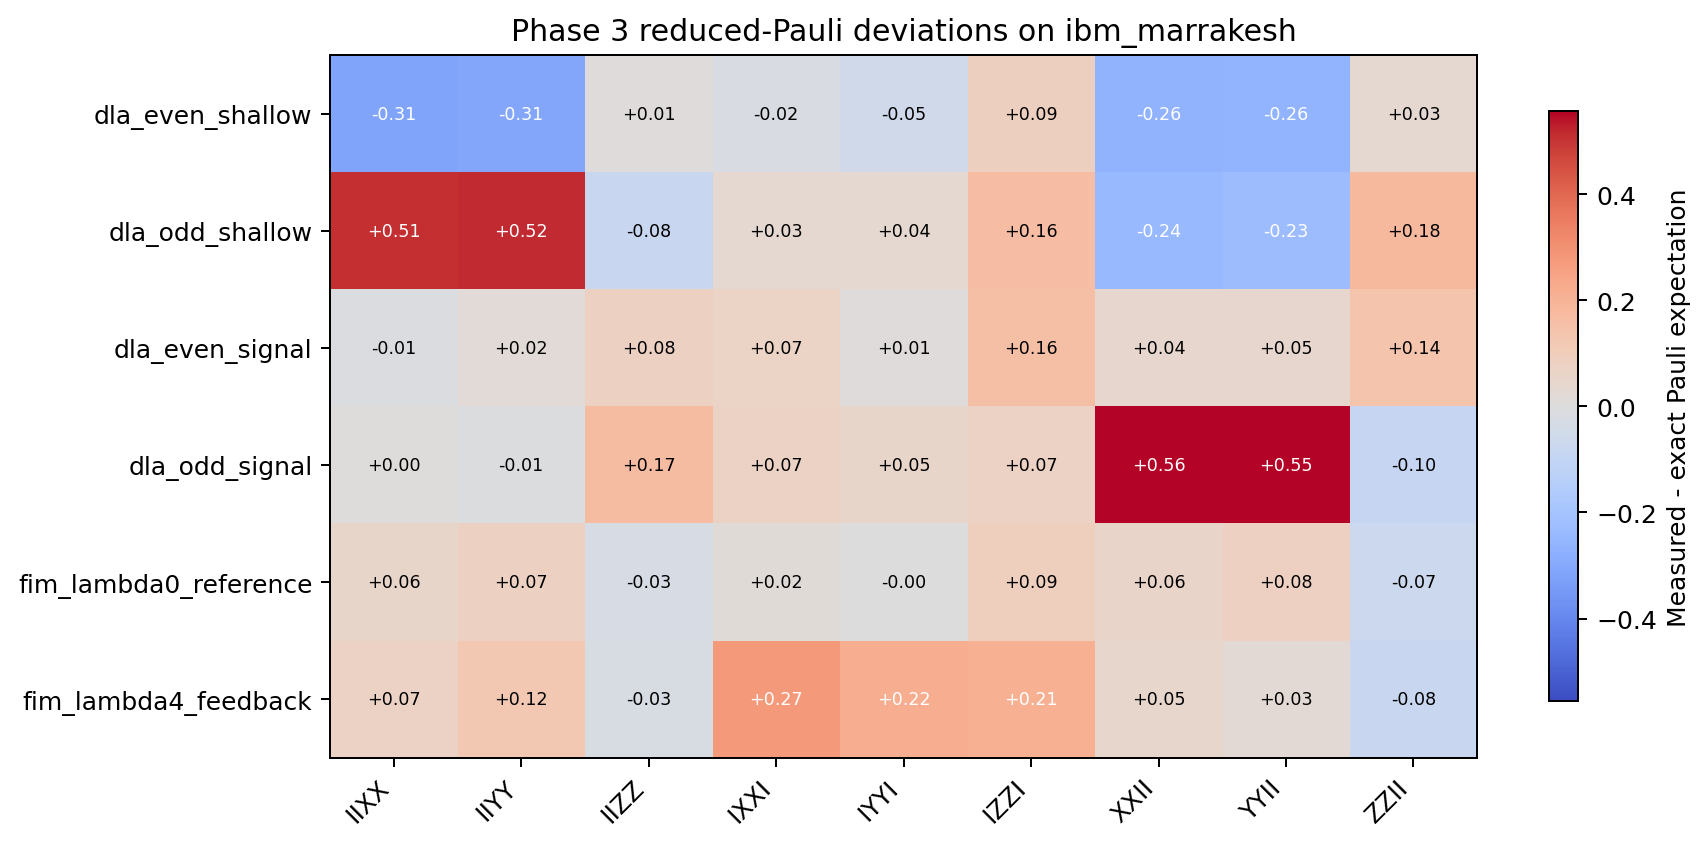
\includegraphics[width=0.98\linewidth]{../../figures/phase3/phase3_entanglement_deviation_heatmap_2026-05-20.png}
\caption{Measured-minus-exact reduced-Pauli deviations for the completed
\texttt{ibm\_marrakesh} run. The strongest deviations concentrate in
transverse edge correlators rather than in all observables uniformly.}
\label{fig:heatmap}
\end{figure}

The largest individual deviations are shown in Table~\ref{tab:top}. The top
four are DLA odd-sector transverse correlators. The strongest FIM-channel
departure is the \texttt{IXXI} observable for the
$\lambda_{\mathrm{fim}}=4$ circuit.

\begin{table}[tb]
\centering
\small
\begin{tabular}{llrrr}
\toprule
Circuit label & Basis & Measured & Exact & Deviation \\
\midrule
\texttt{dla\_odd\_signal} & \texttt{XXII} & 0.431641 & -0.124450 & 0.556091 \\
\texttt{dla\_odd\_signal} & \texttt{YYII} & 0.429688 & -0.124450 & 0.554138 \\
\texttt{dla\_odd\_shallow} & \texttt{IIYY} & 0.488932 & -0.026541 & 0.515473 \\
\texttt{dla\_odd\_shallow} & \texttt{IIXX} & 0.478841 & -0.026541 & 0.505382 \\
\texttt{dla\_even\_shallow} & \texttt{IIXX} & -0.456055 & -0.141874 & -0.314180 \\
\texttt{dla\_even\_shallow} & \texttt{IIYY} & -0.447591 & -0.141874 & -0.305717 \\
\texttt{fim\_lambda4\_feedback} & \texttt{IXXI} & 0.175781 & -0.098373 & 0.274155 \\
\bottomrule
\end{tabular}
\caption{Largest measured-minus-exact deviations in the reduced-Pauli rows.}
\label{tab:top}
\end{table}

\section{Discussion}

The main result is not that the hardware reproduces the exact reduced-Pauli
reference structure. It does not. The contribution is that the departures from
the exact reference are large, structured, and concentrated in specific
correlator channels. This turns the earlier leakage/retention observations
into a sharper hardware-mechanism question: the same circuit families that show
sector-sensitive survival behaviour also show measurable correlator-level
distortions.

The DLA circuits dominate the strongest deviations. The sign structure is
particularly important: odd-sector circuits show large positive transverse
edge-correlator shifts, whereas the even shallow circuit shows large negative
shifts on corresponding channels. This is not consistent with a single scalar
decoherence factor multiplying every observable equally. It is more naturally
read as a sector- and edge-dependent deformation under the selected backend,
layout, circuit family, and calibration window.

The FIM result is more muted but still useful. The $\lambda_{\mathrm{fim}}=4$
feedback circuit deviates more strongly than the $\lambda_{\mathrm{fim}}=0$
reference. This is consistent with the earlier negative fixed-FIM hardware
result: the tested digital FIM modification does not simply protect the target
structure and introduces a measurable reduced-Pauli distortion channel. The
result motivates adaptive FIM follow-up only under a conservative claim
boundary; it does not rescue a fixed-$\lambda_{\mathrm{fim}}$ protection claim.

The readout boundary remains central. Four readout calibration states are
included in the execution block, but the manuscript-level conclusion is based
on unmitigated measured correlators compared with exact references. Because
the largest deviations occur in transverse basis-rotated measurements, not
only in computational-basis \texttt{ZZ} channels, the result is unlikely to be
a pure population-readout story. It may still include basis-rotation error,
layout-dependent coherent error, calibration drift, and depth-dependent
decoherence. The safe interpretation is therefore mechanism-boundary evidence,
not full causal attribution.

\subsection{Readout-sensitivity check}

The four readout calibration circuits provide a scale check for the largest
reduced-Pauli deviations. The dominant measured bitstring for each calibration
state is shown in Table~\ref{tab:readout}. Because Qiskit reports classical
bitstrings with endianness opposite to the source labels for some prepared
states, the table reports the dominant observed bitstring rather than treating
the printed label as a direct left-to-right comparator. The mean dominant-state
retention across the four calibration circuits is 0.9771, corresponding to a
mean leakage from the dominant calibration bitstring of 0.0229. The weakest
calibration state retains 0.9744 of shots.

\begin{table}[tb]
\centering
\small
\begin{tabular}{lrr}
\toprule
Prepared label & Dominant observed bitstring & Retention \\
\midrule
\texttt{0000} & \texttt{0000} & 0.981079 \\
\texttt{0001} & \texttt{1000} & 0.975342 \\
\texttt{0011} & \texttt{1100} & 0.977661 \\
\texttt{1111} & \texttt{1111} & 0.974365 \\
\bottomrule
\end{tabular}
\caption{Readout calibration dominant-state retention for the completed
\texttt{ibm\_marrakesh} execution. The largest reduced-Pauli deviations in
Table~\ref{tab:top} are roughly an order of magnitude larger than this
dominant-bitstring readout leakage scale.}
\label{tab:readout}
\end{table}

This calibration block does not remove the need for caution: transverse
basis-rotated measurements can be affected by basis-rotation and coherent gate
errors before readout. It does, however, make a pure computational-basis
readout-retention explanation implausible for the largest observed effects.
The maximum reduced-Pauli deviation, 0.5561, is about 21.7 times the worst
dominant-state calibration leakage of 0.0256 and about 24.3 times the mean
dominant-state calibration leakage of 0.0229. The paper's claim boundary is
therefore refined as follows: readout calibration does not by itself explain
the largest transverse correlator deviations, but the result remains a
compound hardware-window observation rather than an isolated entanglement
mechanism attribution.

\section{Claim boundary}

The supported claims are intentionally narrow. The run measured preregistered
reduced-Pauli correlators for small Kuramoto--XY DLA and FIM circuit families
on one IBM Heron backend and layout. The measured correlators deviate from
exact references in a structured way, with the largest deviations in
transverse edge channels. This constrains the mechanism interpretation of the
earlier DLA/FIM hardware programme.

The result does not support quantum advantage, scalable tomography, full-state
reconstruction, backend-general entanglement dynamics, or claims about
unmeasured circuits, depths, layouts, or backends.

\section{Reproducibility}

The source code and data are in the
\href{https://github.com/anulum/scpn-quantum-control}{\texttt{anulum/scpn-quantum-control}}
repository. The relevant commands are:
\begin{itemize}
  \item live readiness and gated submission:
    \path{scripts/phase3_entanglement_tomography_ibm.py};
  \item completed raw-count artefact:
    \path{data/phase3_entanglement_tomography/entanglement_tomography_live_ibm_marrakesh_2026-05-20T004334Z.json};
  \item post-run reducer:
    \path{scripts/analyse_phase3_entanglement_tomography.py};
  \item paper-asset generator:
    \path{scripts/generate_phase3_entanglement_paper_assets.py}.
\end{itemize}

\section{Conclusion}

A preregistered 166-circuit IBM Heron run measured 54 reduced-Pauli observables
for promoted DLA and FIM Kuramoto--XY circuits. The resulting deviations from
exact references are large and structured, with the strongest departures in
transverse DLA edge correlators and a smaller but clear FIM
$\lambda_{\mathrm{fim}}=4$ distortion. The paper's contribution is a bounded
mechanism-separation result: it localises correlator-level hardware
deformation accompanying the earlier leakage/retention observations and shows
that the largest effects exceed the dominant computational-basis readout
leakage scale. It still avoids scalable tomography, backend-general,
full-causal-entanglement, or advantage claims.

\bibliographystyle{apsrev4-2}
\bibliography{phase3_entanglement_tomography_refs}

\end{document}
